% Primes the Tectonic cache with the packages and font sizes that generated
% reports use, so `just latex::render` can build them from cached resources only.
\documentclass[10pt]{article}
\usepackage[margin=2cm]{geometry}
\usepackage[T1]{fontenc}
\usepackage{lmodern}
\usepackage{booktabs}
\usepackage{pgfplots}
\pgfplotsset{compat=1.18}
\title{Report}
\author{}
\date{}
\begin{document}
\maketitle
\section{Section}
\subsection{Subsection}
{\tiny a \textbf{b} \emph{c} $x \geq \kappa \times y_1^2$}
{\scriptsize a \textbf{b} \emph{c} $x \geq \kappa \times y_1^2$}
{\footnotesize a \textbf{b} \emph{c} $x \geq \kappa \times y_1^2$}
{\small a \textbf{b} \emph{c} $x \geq \kappa \times y_1^2 \leq z$}
{\normalsize a \textbf{b} \emph{c} $x \geq \kappa \times y_1^2 \leq z$}
{\large a \textbf{b}} {\Large a \textbf{b}} {\LARGE a} {\huge a}
{\fontencoding{OT1}\selectfont
  {\tiny a \textbf{b} \emph{c}} {\scriptsize a \textbf{b} \emph{c}}
  {\footnotesize a \textbf{b} \emph{c}} {\small a \textbf{b} \emph{c}}
  {\normalsize a \textbf{b} \emph{c}} {\large a} {\Large a}}
\begin{table}[h]\centering\small
  \begin{tabular}{lr}\toprule A & B \\ \midrule 1 & 2 \\ \bottomrule\end{tabular}
  \caption{Table.}
\end{table}
\begin{figure}[h]\centering
  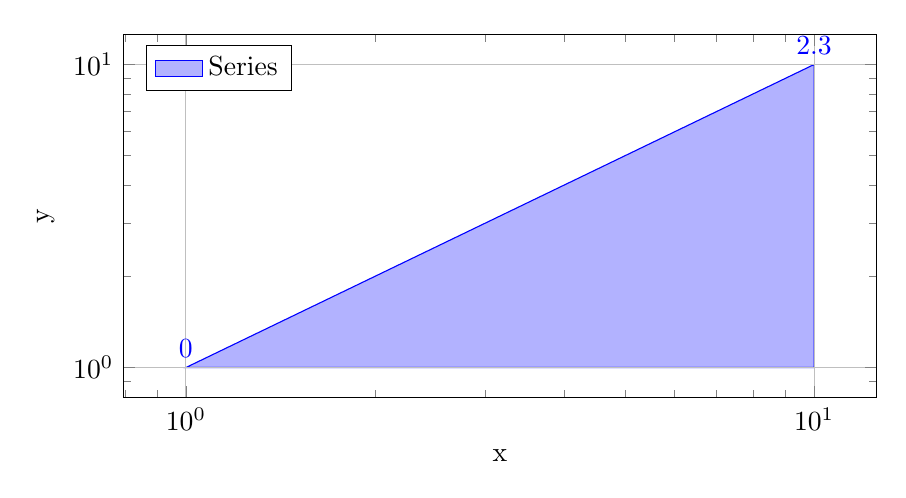
\begin{tikzpicture}
    \begin{axis}[width=0.92\linewidth, height=6.2cm, grid=major, xmode=log,
        ymode=log, stack plots=y, area style, legend pos=north west,
        nodes near coords, xlabel={x}, ylabel={y}]
      \addplot coordinates {(1,1) (10,10)} \closedcycle;
      \addlegendentry{Series}
    \end{axis}
  \end{tikzpicture}
  \caption{Figure.}
\end{figure}
\end{document}
